\message{ !name(paper.tex)}\documentclass[10pt,twocolumn,letterpaper]{article}

\usepackage{cvpr} \usepackage{times} \usepackage{epsfig}
\usepackage{graphicx} \usepackage{amsmath} \usepackage{amssymb}
\usepackage{subfig}

% Include other packages here, before hyperref.

% If you comment hyperref and then uncomment it, you should delete
% egpaper.aux before re-running latex.  (Or just hit 'q' on the first
% latex run, let it finish, and you should be clear).
\usepackage[pagebackref=true,breaklinks=true,letterpaper=true,colorlinks,bookmarks=false]{hyperref}


% \cvprfinalcopy % *** Uncomment this line for the final submission

\def\cvprPaperID{****} % *** Enter the 3DIMPVT Paper ID here
\def\httilde{\mbox{\tt\raisebox{-.5ex}{\symbol{126}}}}

% Pages are numbered in submission mode, and unnumbered in
% camera-ready
\ifcvprfinal\pagestyle{empty}\fi
\begin{document}

\message{ !name(paper.tex) !offset(171) }
\begin{figure}
  \centering
  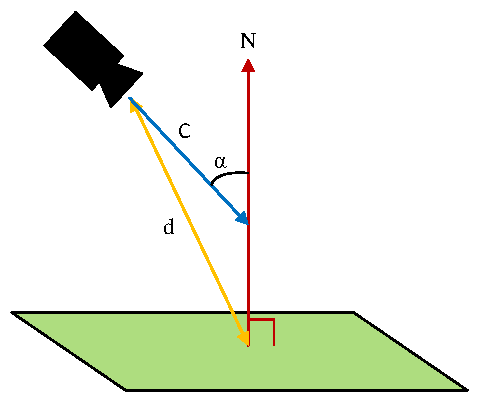
\includegraphics[height=1.5in]{scoringFunction.pdf}
  \caption{We wish to minimize camera angle $\alpha$ and distance $d$}
  \label{fig:scoringFunction}
\end{figure}
\message{ !name(paper.tex) !offset(712) }

\end{document}
